% The generative chain: (mu, omega) to a row of reported statistics.
% Boustrophedon layout -- top row left to right, elbow at the right, bottom row
% right to left -- so the whole chain fits a slide without a long return arrow.
%
%   compile:  pdflatex generative_chain.tex
%   output :  generative_chain.pdf
%
\documentclass[border=10pt]{standalone}
\usepackage{lmodern}
\usepackage{amsmath}
\usepackage{amssymb}
\usepackage{tikz}
\usetikzlibrary{arrows.meta,positioning,calc}
% Shared palette for the population-model figures.
%   ink      body / structure
%   popcol   the patient cloud and anything predicted from it
%   mechcol  the simulator and species-level quantities
%   msrcol   the measurement map (readout-level: gamma, kappa)
%   datacol  reported rows
\definecolor{ink}{HTML}{3A3A3A}
\definecolor{popcol}{HTML}{3B4AA6}
\definecolor{mechcol}{HTML}{2E7D5B}
\definecolor{msrcol}{HTML}{EB811B}
\definecolor{datacol}{HTML}{8C3B4A}

\newcommand{\Ncal}{\mathcal{N}}

\begin{document}
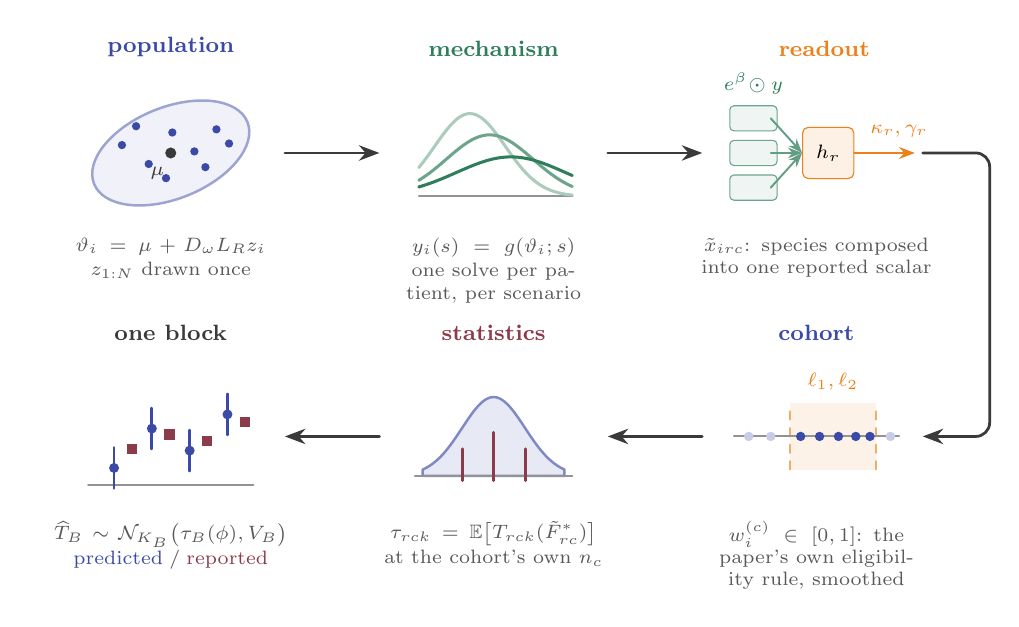
\begin{tikzpicture}[
  font=\sffamily, >=Stealth, line cap=round, line join=round,
  stagelab/.style={font=\footnotesize\bfseries, anchor=south},
  eqlab/.style={font=\scriptsize, anchor=north, text=ink!85, align=center,
                text width=34mm},
  fl/.style={-{Stealth[length=2.6mm]}, ink, line width=1pt}]

\def\dx{4.1}

% ================================================================ row 1
% ---- (A) the patient cloud -------------------------------------------
\begin{scope}[shift={(0,0)}]
  \draw[popcol!50, fill=popcol!7, line width=0.9pt, rotate=22] (0,0) ellipse (1.05 and 0.58);
  \foreach \p in {(-0.62,0.10),(-0.28,-0.14),(0.02,0.26),(0.30,0.02),(0.58,0.30),
                  (-0.06,-0.32),(0.44,-0.18),(0.74,0.12),(-0.44,0.34)}
    \fill[popcol] \p circle (1.5pt);
  \fill[ink] (0,0) circle (2pt);
  \node[ink, font=\scriptsize, anchor=north east] at (0.04,-0.05) {$\mu$};
  \node[stagelab, popcol] at (0,1.10) {population};
\end{scope}
\node[eqlab] at (0,-0.95) {$\vartheta_i=\mu+D_\omega L_R z_i$\\[1pt] $z_{1:N}$ drawn once};

\draw[fl] (1.45,0) -- (2.65,0);

% ---- (B) the simulator ------------------------------------------------
\begin{scope}[shift={(\dx,0)}]
  \draw[ink!55, line width=0.7pt] (-0.95,-0.55) -- (1.0,-0.55);
  \draw[mechcol!40, line width=1.1pt]
    plot[domain=-0.95:1.0,samples=60,smooth] (\x,{-0.55+1.05*exp(-(\x+0.30)*(\x+0.30)/0.40)});
  \draw[mechcol!70, line width=1.1pt]
    plot[domain=-0.95:1.0,samples=60,smooth] (\x,{-0.55+0.78*exp(-(\x+0.05)*(\x+0.05)/0.60)});
  \draw[mechcol, line width=1.1pt]
    plot[domain=-0.95:1.0,samples=60,smooth] (\x,{-0.55+0.50*exp(-(\x-0.22)*(\x-0.22)/0.95)});
  \node[stagelab, mechcol] at (0,1.10) {mechanism};
\end{scope}
\node[eqlab] at (\dx,-0.95) {$y_i(s)=g(\vartheta_i;s)$\\[1pt] one solve per patient, per scenario};

\draw[fl] ({\dx+1.45},0) -- ({\dx+2.65},0);

% ---- (C) readout + discrepancy ---------------------------------------
\begin{scope}[shift={(2*\dx,0)}]
  \foreach \y in {0.44,0.00,-0.44}
    \node[draw=mechcol!70, fill=mechcol!8, rounded corners=1.5pt,
          minimum width=6mm, minimum height=3.2mm, inner sep=0pt] at (-0.80,\y) {};
  \node[draw=msrcol, fill=msrcol!12, rounded corners=2pt, minimum size=6.5mm,
        inner sep=1pt, font=\scriptsize] (hr) at (0.15,0) {$h_r$};
  \foreach \y in {0.44,0.00,-0.44}
    \draw[mechcol!75, -{Stealth[length=1.8mm]}, line width=0.7pt] (-0.58,\y) -- (hr.west);
  \draw[msrcol, -{Stealth[length=2mm]}, line width=0.9pt] (hr.east) -- (1.25,0);
  \node[font=\scriptsize, mechcol, anchor=south] at (-0.80,0.62) {$e^{\beta}\!\odot y$};
  \node[font=\scriptsize, msrcol, anchor=south west] at (0.56,0.08) {$\kappa_r,\gamma_r$};
  \node[stagelab, msrcol] at (0.1,1.10) {readout};
\end{scope}
\node[eqlab] at (2*\dx,-0.95) {$\tilde x_{irc}$: species composed into one reported scalar};

% ---- elbow ------------------------------------------------------------
\draw[fl, rounded corners=5pt]
  ({2*\dx+1.35},0) -- ({2*\dx+2.20},0) -- ({2*\dx+2.20},-3.6) -- ({2*\dx+1.35},-3.6);

% ================================================================ row 2
% ---- (D) cohort selection --------------------------------------------
\begin{scope}[shift={(2*\dx,-3.6)}]
  \fill[msrcol!10] (-0.34,-0.42) rectangle (0.76,0.42);
  \draw[msrcol!65, dashed, line width=0.7pt] (-0.34,-0.42) -- (-0.34,0.42);
  \draw[msrcol!65, dashed, line width=0.7pt] (0.76,-0.42) -- (0.76,0.42);
  \draw[ink!55, line width=0.7pt] (-1.05,0) -- (1.05,0);
  \foreach \x in {-0.86,-0.58,0.94} \fill[popcol!28] (\x,0) circle (1.7pt);
  \foreach \x in {-0.20,0.04,0.28,0.50,0.68} \fill[popcol] (\x,0) circle (1.7pt);
  \node[font=\scriptsize, msrcol, anchor=south] at (0.21,0.46) {$\ell_1,\ell_2$};
  \node[stagelab, popcol] at (0,1.10) {cohort};
\end{scope}
\node[eqlab] at (2*\dx,-4.55) {$w^{(c)}_i\in[0,1]$: the paper's own eligibility rule, smoothed};

\draw[fl] ({\dx+2.65},-3.6) -- ({\dx+1.45},-3.6);

% ---- (E) statistics ---------------------------------------------------
\begin{scope}[shift={(\dx,-3.6)}]
  \draw[popcol!65, fill=popcol!12, line width=0.9pt]
    plot[domain=-0.90:0.90,samples=70,smooth] (\x,{-0.50+1.00*exp(-\x*\x/0.32)})
    -- (0.90,-0.50) -- (-0.90,-0.50) -- cycle;
  \draw[ink!55, line width=0.7pt] (-1.00,-0.50) -- (1.00,-0.50);
  \foreach \x/\h in {-0.40/0.62, 0.00/1.00, 0.40/0.62}
    \draw[datacol, line width=1.1pt] (\x,-0.56) -- (\x,{-0.50+\h*0.55});
  \node[stagelab, datacol] at (0,1.10) {statistics};
\end{scope}
\node[eqlab] at (\dx,-4.55) {$\tau_{rck}=\mathbb{E}\big[T_{rck}(\tilde F^{\ast}_{rc})\big]$\\[1pt]
  at the cohort's own $n_c$};

\draw[fl] (2.65,-3.6) -- (1.45,-3.6);

% ---- (F) the comparison ----------------------------------------------
\begin{scope}[shift={(0,-3.6)}]
  \draw[ink!55, line width=0.7pt] (-1.05,-0.62) -- (1.05,-0.62);
  \foreach \x/\p in {-0.72/0.22, -0.24/0.72, 0.24/0.44, 0.72/0.90}{
    \draw[popcol, line width=1pt] (\x,{-0.62+\p-0.26}) -- (\x,{-0.62+\p+0.26});
    \fill[popcol] (\x,{-0.62+\p}) circle (1.8pt);}
  \foreach \x/\p in {-0.72/0.40, -0.24/0.58, 0.24/0.50, 0.72/0.74}
    \fill[datacol] ({\x+0.16},{-0.62+\p}) rectangle ({\x+0.29},{-0.62+\p+0.13});
  \node[stagelab, ink] at (0,1.10) {one block};
\end{scope}
\node[eqlab] at (0,-4.55) {$\widehat T_B\sim\Ncal_{K_B}\big(\tau_B(\phi),V_B\big)$\\[1pt]
  \textcolor{popcol}{predicted}\;/\;\textcolor{datacol}{reported}};

\end{tikzpicture}
\end{document}
